\documentclass[conference]{IEEEtran}
\IEEEoverridecommandlockouts
\usepackage{amsmath,amssymb,amsfonts}
\usepackage{algorithmic}
\usepackage{caption}
\usepackage{cite}
\usepackage{graphicx}
\usepackage{textcomp}
\usepackage{xcolor}
\def\BibTeX{{\rm B\kern-.05em{\sc i\kern-.025em b}\kern-.08em
    T\kern-.1667em\lower.7ex\hbox{E}\kern-.125emX}}
\begin{document}

\title{Enhanced Quantitative Trading Strategies through Sentiment Analysis Using Large Language Models}

\author{
    \IEEEauthorblockN{1\textsuperscript{st} Wentao Ye}
    \IEEEauthorblockA{\textit{SIGS} \\
    \textit{Tsinghua University}\\
    Shenzhen, China \\
    yewt23@mails.tsinghua.edu.cn}
    \and
    \IEEEauthorblockN{2\textsuperscript{nd} Huaxuan Li}
    \IEEEauthorblockA{\textit{SIGS} \\
    \textit{Tsinghua University}\\
    Shenzhen, China \\
    lhx23@mails.tsinghua.edu.cn}
    \and
    \IEEEauthorblockN{3\textsuperscript{rd} Jiadong Li}
    \IEEEauthorblockA{\textit{SIGS} \\
    \textit{Tsinghua University}\\
    Shenzhen, China \\
    lijd23@mails.tsinghua.edu.cn}
    \thanks{W. Ye designed the workflow, deployed and fine-tuned the language models, developed the trading strategies, performed data analysis and wrote the manuscript.
    H. Li conducted the related work review, forecast model selection, backtesting and wrote the poster.
    J. Li conducted interference of LLM and integrated the sentiment analysis with traditional price-volume features.
    All authors contributed to the design of the study.
    }
    \thanks{Acknowledgment: This work was supported by Jiachen Wang, Wentao Ye, Rui Chen and Hanyu Wei, who provided valuable computational resources. 
    We also thank Qlib project in Microsoft Research Asia for providing the open source quantitative investment platform and Llama project in Meta AI for providing the pre-trained language models.}
}

\maketitle

\begin{abstract}
The stock market's significant price volatility necessitates sophisticated and adaptive trading strategies. 
Traditional quantitative trading strategies relying on numerical data often overlook psychological factors from investors.
This project integrates sentiment analysis using large language models (LLMs) to enhance quantitative trading strategies. 
By incorporating sentiment analysis from news articles and social media, we aim to improve trading performance, decision-making accuracy, and overall profitability in quantitative trading.
\end{abstract}

\begin{IEEEkeywords}
Quantitative Finance, Sentiment Analysis, Large Language Models, Stock Market, Trading Strategies
\end{IEEEkeywords}

\section{\textbf{Introduction}}

The stock market is characterized by its significant price volatility driven by factors such as market sentiment, speculative trading, and news events. 
This volatility creates opportunities for profit but also introduces risk, necessitating sophisticated trading strategies.

Traditional strategies rely on historical data and often neglect psychological factors from investors. 
With the rise of social media and news platforms, lagre amount of unstructured data from social media and news can provide valuable insights into market sentiment and trends, which are not captured by traditional quantitative strategies.

Large language models (LLMs) have revolutionized natural language processing (NLP) tasks, achieving state-of-the-art performance in various domains, it can be fine-tuned for specific tasks, such as sentiment analysis, to extract valuable insights from textual data, which provides a promising approach to enhance quantitative trading strategies.

\section{\textbf{Ralated Work}}

\subsection{\textbf{Qlib}}
Qlib is an AI-oriented quantitative investment platform that provides a comprehensive set of tools for quantitative trading strategies, including data processing, feature engineering, model training, and backtesting, to facilitate the development of quantitative trading strategies \cite{yang2020}.

\subsection{\textbf{Sentiment Analysis with Large Language Models}}
Recent studies have explored the application of LLMs in sentiment analysis tasks, such as financial news analytics and market sentiment analysis.
Deng et al. investigated the use of LLMs for Reddit market sentiment analysis, demonstrating the effectiveness of LLMs in capturing market sentiment from social media data \cite{deng2023}.
Pavlyshenko proposed a fine-tuned Llama 2 GPT model for financial news analytics, highlighting the model's ability to extract valuable insights from financial news data \cite{pavlyshenko2023}.
These studies demonstrate the potential of LLMs in sentiment analysis tasks and their application in financial markets.

\section{\textbf{Method}}
\subsection{\textbf{Overview of the Workflow}}

Our project integrates sentiment analysis with traditional price-volume trading strategies to enhance quantitative trading strategies.
The workflow consists of three main components: Information Extraction, Decision Generation, and Execution. 
The workflow is illustrated in Fig. \ref{fig:workflow}.

\begin{figure}[htbp]
    \centering
    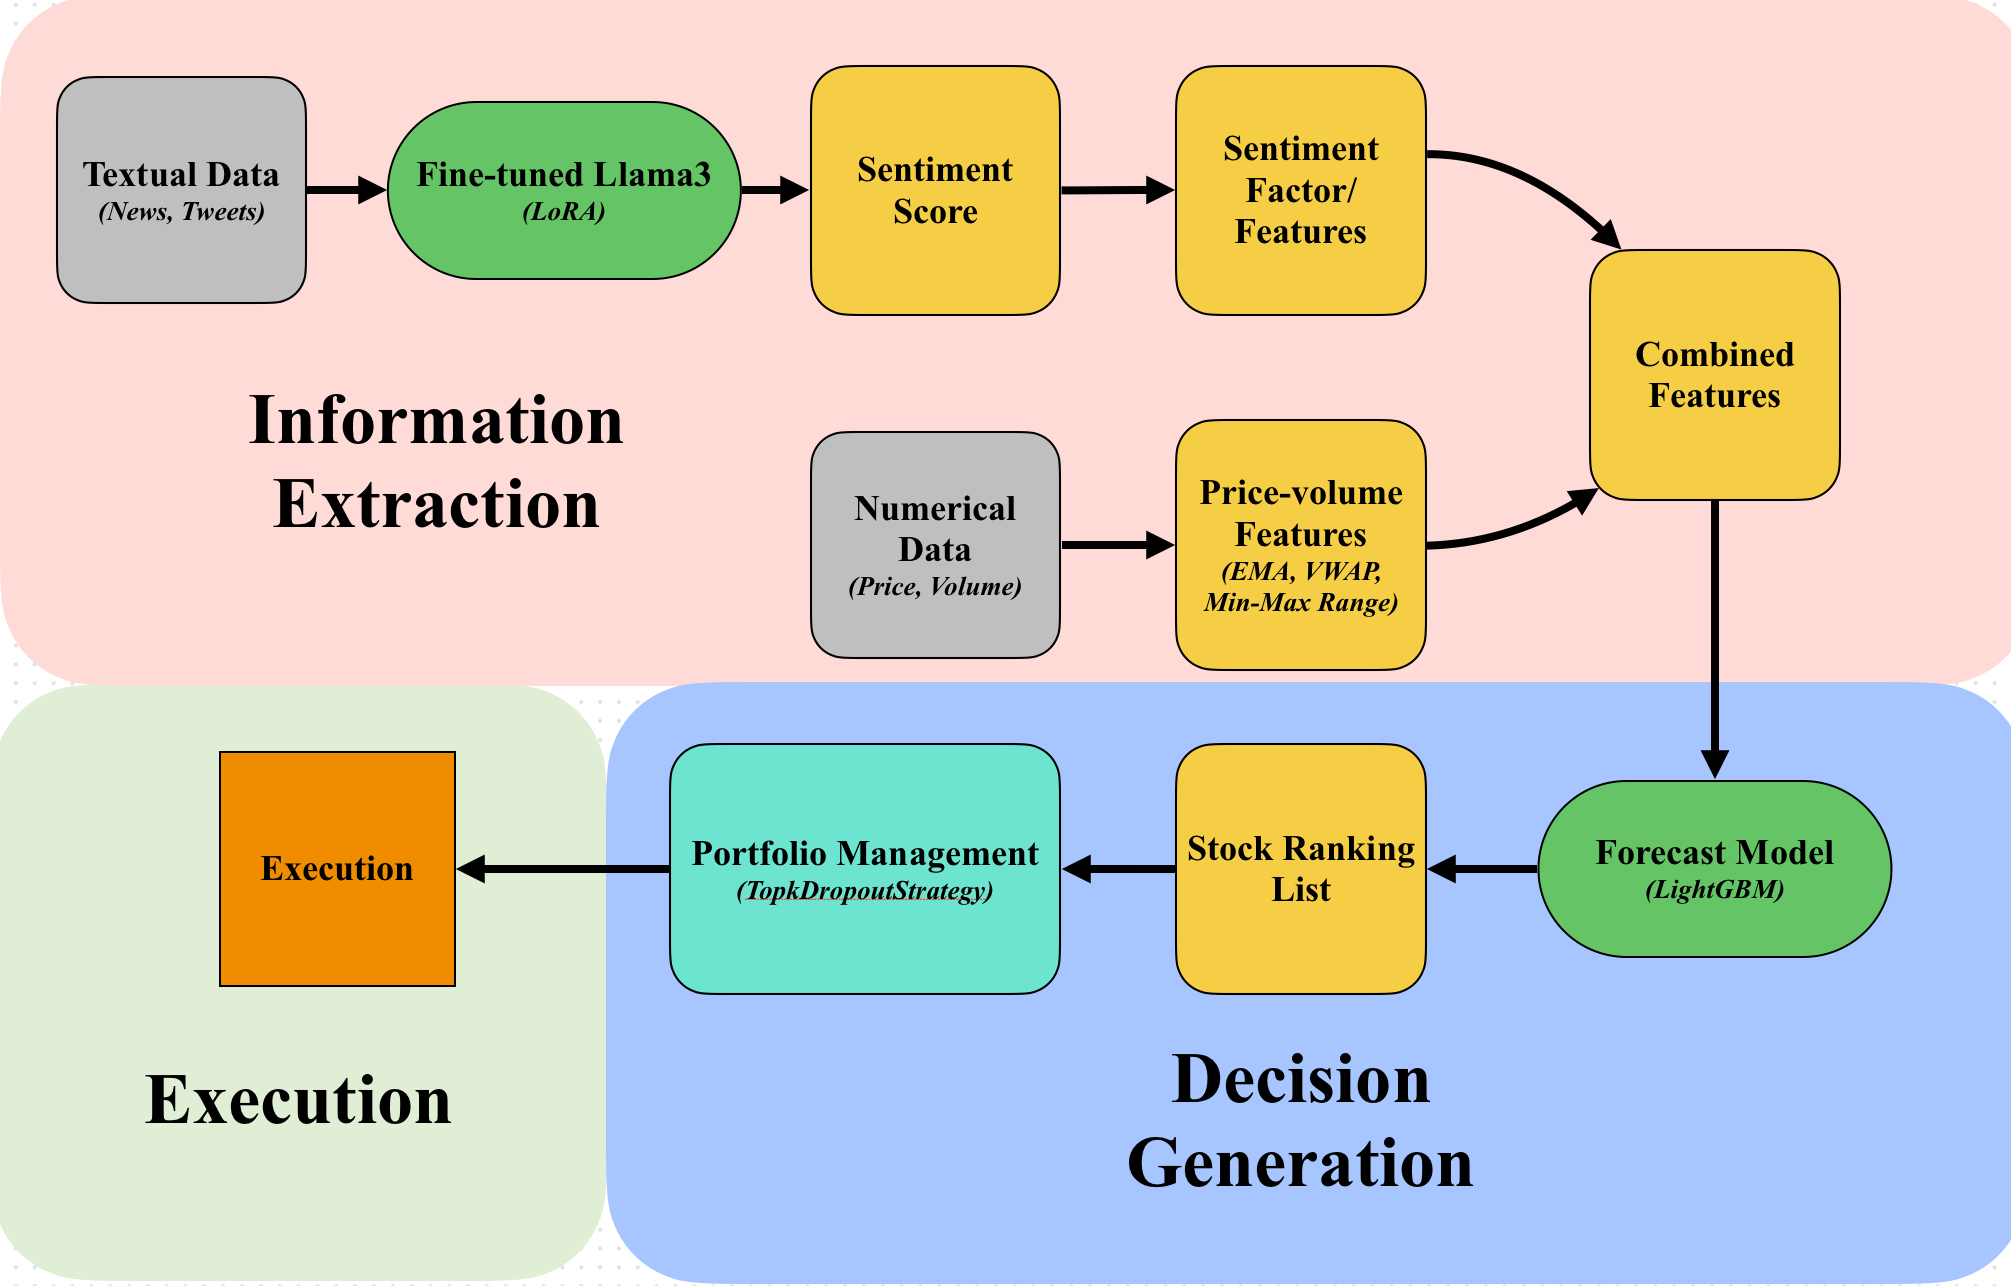
\includegraphics[width=0.3\textwidth]{workflow.jpg}
    \caption{Quantitative Trading Strategies with Sentiment Analysis Workflow.}
    \label{fig:workflow}
\end{figure}

\subsubsection{Information Extraction}

This stage involves gathering and processing both textual and numerical data to generate actionable factors for trading models.

\paragraph{Textual Data Processing:}
\begin{itemize}
    \item \textbf{Data Source:} Textual data is sourced from news articles and social media platforms such as Twitter.
    \item \textbf{Sentiment Scoring:} The fine-tuned Llama 3 model generates sentiment scores from the textual data, reflecting market sentiment towards various stocks or market conditions.
    \item \textbf{Sentiment Factor:} These sentiment scores are then transformed into sentiment factors, which are used as input features for the trading model.
\end{itemize}

\paragraph{Numerical Data Processing:}
\begin{itemize}
    \item \textbf{Data Source:} Numerical data includes price and volume information for various stocks.
    \item \textbf{Price-Volume Features:} Key features such as Exponential Moving Average (EMA), and Min-Max Range are derived from the numerical data. These factors capture essential market dynamics and trends.
\end{itemize}

\paragraph{Combined Features Creation:}
\begin{itemize}
    \item \textbf{Integration:} Sentiment factors and price-volume features are combined to form a comprehensive set of input features for the trading model. This integrated approach allows the model to consider both market sentiment and quantitative metrics.
\end{itemize}

\subsubsection{Decision Generation}

In this stage, the derived features are used to generate trading signals and manage the portfolio.

\paragraph{Forecast Model:}
\begin{itemize}
    \item \textbf{Model Selection:} We utilize the LightGBM model, a gradient boosting framework, to forecast future price movements and generate trading signals based on the combined features.
    \item \textbf{Stock Ranking List:} The LightGBM model ranks the stocks, indicating which stocks are likely to perform well based on the input features.
\end{itemize}

\paragraph{Portfolio Management:}
\begin{itemize}
    \item \textbf{Strategy Implementation:} \texttt{TopkDropoutStrategy} is used to manage the portfolio. This strategy involves buying and selling a fixed number of stocks daily based on their ranked trading signals.
\end{itemize}

\subsubsection{Execution}

The final component involves executing the trading decisions generated in the previous stage.

\subsection{\textbf{Information Extraction}}

\subsubsection{\textbf{LLM Fine-Tuning Methods Based on Sentiment Data}}
In our project, we leverage LoRA to fine-tune Llama 3, a state-of-the-art large language model.
Fine-tuning improves the LLM model's performance in specific tasks, such as sentiment analysis, by adapting it to domain-specific data.
Traditional fine-tuning of models like Llama 3 can be computationally expensive and resource-intensive. 
LoRA, a parameter-efficient fine-tuning (PEFT) method, addresses this challenge by freezing the pre-trained model weights and injecting trainable rank decomposition matrices into each layer of the Transformer architecture, greatly reducing the number of trainable parameters for downstream tasks, making the fine-tuning process faster and less resource-demanding, but still maintains high performance in task-specific adjustments \cite{hu2021}.
Specifically, the fine-tuning process starts by initializing the pre-trained Llama 3 model. 
The pre-trained weights provide a solid foundation, having been trained on diverse and extensive corpus data. 
LoRA layers are then integrated into Llama 3. 
These layers are low-rank matrices that capture task-specific adjustments, minimizing computational costs by introducing low-rank matrices \( A \in \mathbb{R}^{d \times r} \) and \( B \in \mathbb{R}^{r \times k} \) to approximate the original weight matrix \( W \in \mathbb{R}^{d \times k} \), where \( r \) is the rank of the decomposition, and \( r \ll \min(d, k) \).
Instead of updating all model parameters, LoRA adds the product of these matrices to the original weight matrix \( W \), as \( W' = W + A \times B \). 
During the fine-tuning process, only the matrices \(A\) and \(B\) are trained, which significantly reduces the number of parameters to be updated, making the process more efficient, as shown in Fig. \ref{fig:lora}.

\begin{figure}[htbp]
    \centering
    \includegraphics[width=0.2\textwidth]{lora.png}
    \caption{The Low-rank Adaptation Method.}
    \label{fig:lora}
\end{figure}

\subsubsection{\textbf{Factor Generated by Sentiment Analysis}}
Once fine-tuned, Llama 3 is integrated into our sentiment analysis pipeline. 
The model processes textual data from news or social media, classifying sentiments accurately and efficiently. 
The estimated sentiment value can therefore be used for generate sentiment factors, where we use explonantial weighted moving average to account for the time decay of the sentiment information.

\subsubsection{\textbf{Features Combination with Traditional Quantitative Features}}
The original price-volume data consists of opening price, closing price, highest price, lowest price, trading volume, and restoration factor. 
With this information, various features can be created.
The features encompass various aspects of market data, technical indicators, and statistical measures, enabling a holistic understanding of market dynamics.

Here we treat the sentiment factor as a new type of feature, and combine it with traditional quantitative price-volume features to create a hybrid feature set.

\subsection{\textbf{Decision Generation}}

We chose LightGBM model as our forecast model, which is a gradient boosting framework based on decision trees. 
During the training process, LightGBM constructs a series of decision trees iteratively, where each tree is built to minimize the residual errors of the previous trees. 
The model ranks features based on their importance scores, which indicate the contribution of each feature to the prediction. 
These importance scores can be used to generate a stock ranking list, displaying the significance of each stock in the model \cite{ke2017}.

After generating the ranking list, we can use a simple rule-based \texttt{TopkDropoutStrategy} to determine the target amount of each stock. 
The strategy adopts the Topk-Drop algorithm, which sells and buys a fixed number of stocks every trading day based on the prediction scores. 
The detailed steps of the \texttt{TopkDropoutStrategy} are as follows:

\begin{itemize}
    \item Adopt the Topk-Drop algorithm to calculate the target amount of each stock.
    
    There are two parameters for the Topk-Drop algorithm:
    \begin{itemize}
        \item \textbf{Topk}: The number of stocks held.
        \item \textbf{Drop}: The number of stocks sold on each trading day.
    \end{itemize}
    
    In general, the number of stocks currently held is \texttt{Topk}, with the exception of being zero at the beginning period of trading. 
    For each trading day, let $d$ be the number of the instruments currently held and with a rank $K$ when ranked by the prediction scores from high to low. 
    Then $d$ number of stocks currently held with the worst prediction score will be sold, and the same number of unheld stocks with the best prediction score will be bought.
    
    In most cases, the Topk-Drop algorithm sells and buys \texttt{Drop} stocks every trading day, which yields a turnover rate of $2 \times \texttt{Drop} / K$.
    
    The following images illustrate a typical scenario.

    \begin{figure}[htbp]
        \centering
        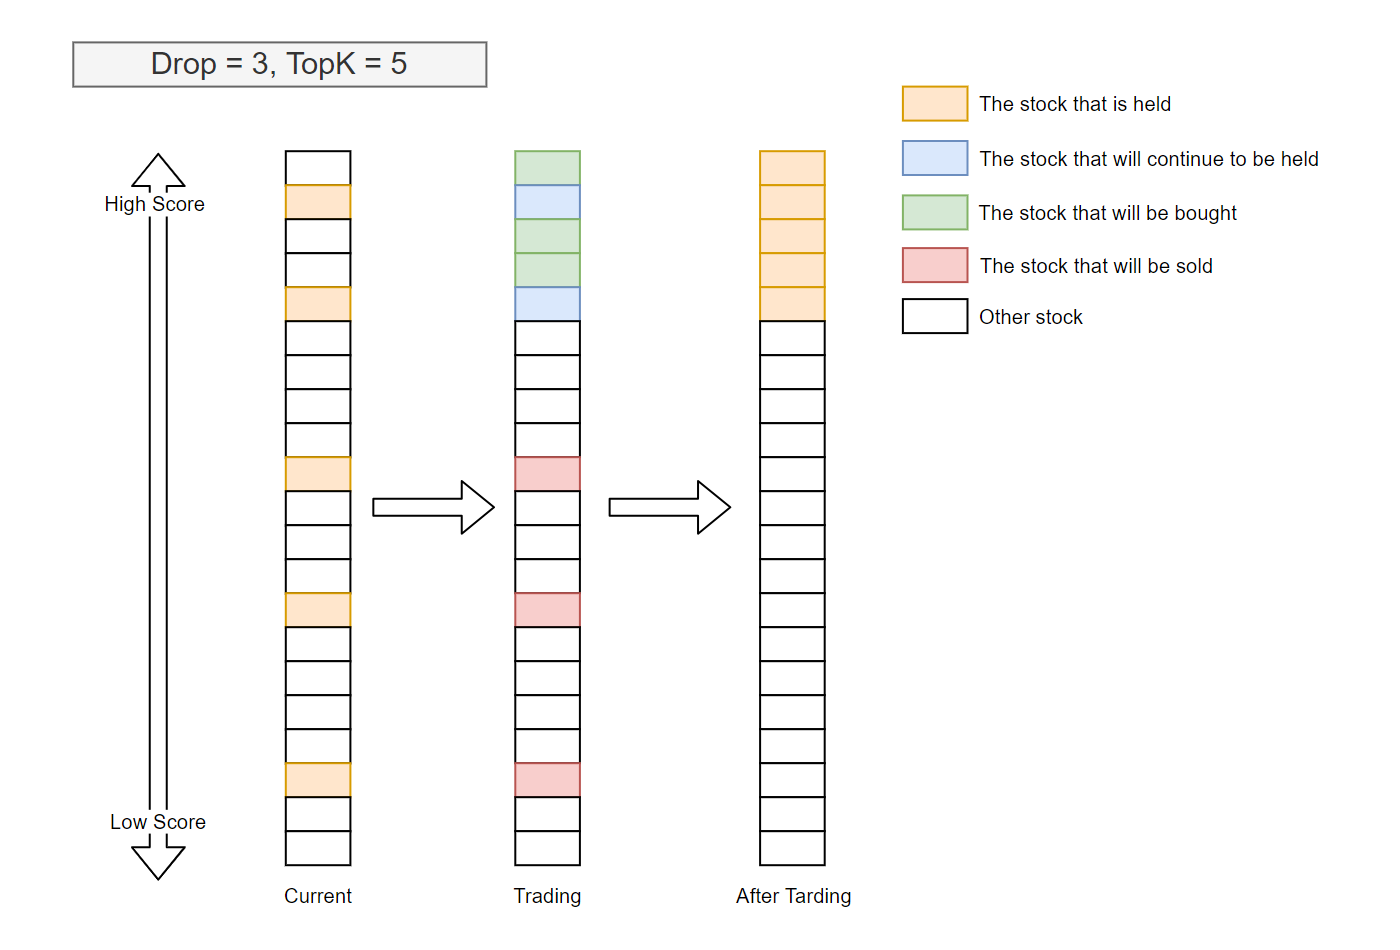
\includegraphics[width=0.3\textwidth]{topk_drop.png}
        \caption{TopkDropoutStrategy}
        \label{fig:TopkDropoutStrategy}
    \end{figure}

    \item Generate the order list from the target amount, and the order list is then sent to the Execution Environment for execution.
\end{itemize}

\section{\textbf{Backtesting Results}}

\subsection{\textbf{Results}}

\begin{itemize}
    \item \textbf{Time Period:} January 1, 2020, to August 1, 2022.
    \item \textbf{Benchmark:} SPY, the SPDR S\&P 500 ETF trust, designed to track the S\&P 500 stock market index.
    \item \textbf{Transaction Cost:} Commission of 0.0005.
\end{itemize}

Our quantitative framework backtested from January 1, 2020, to August 1, 2022, using the SPY as the benchmark.
As shown in Fig. \ref{fig:comprehensive report}, the comprehensive report includes various performance metrics.

\begin{figure}[htbp]
\centering
    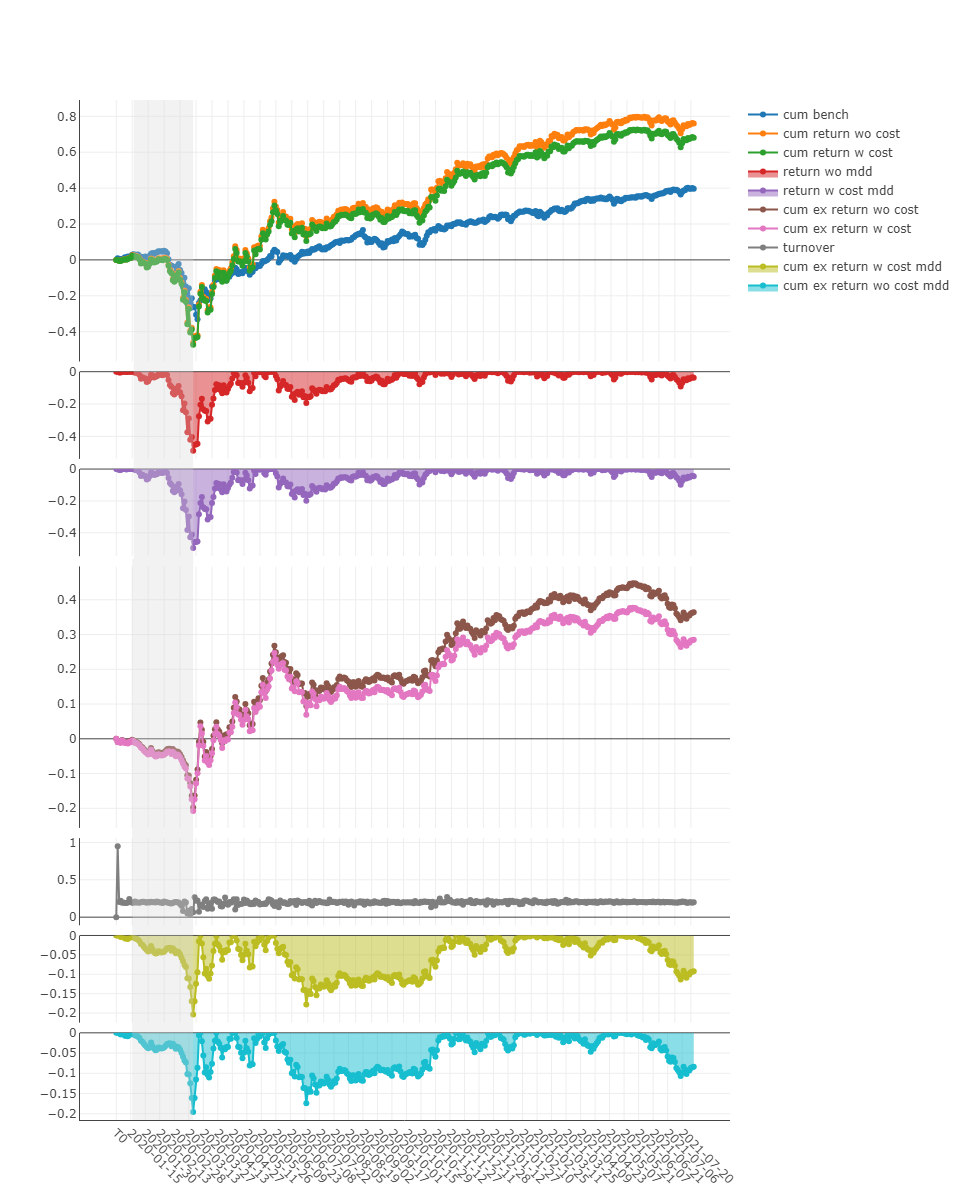
\includegraphics[width=0.4\textwidth]{plot_0.png}
    \caption{Comprehensive Report}
    \captionsetup{justification=raggedright, singlelinecheck=false}
    \caption*{\scriptsize Comment: 'wo' means that without accounting for transaction costs, 'w' means that accounting for transaction costs.
    Besides, 'ex' means that the excess return is calculated by subtracting the benchmark return from the strategy return, 'mdd' means the maximum drawdown, same in the following figures.
    But, 'cum' means cumulative, which is the sum of the daily returns from the start date to the current date, so it's different from the monthly seperated return in the following figures.}
    \label{fig:comprehensive report}
\end{figure}

In January to April 2020, the strategy and benchmark both experienced a significant drawdown, and the strategy even underperformed the benchmark.
We can observe that the strategy's excess return was negative during this period
{\footnote{
\footnotesize{The difference between the 'wo' and 'w' strategies is slight in the early stage. 
Since report shows a cumulative return, we can gradually observe the difference between the two curves with time going on.
But their difference is not significant, so we mainly focus on the 'w' strategy.}
}.
Meanwiile, the strategy's maximum drawdown was about -0.45, which was worse than the benchmark's -0.25, both of which reached the peak in March 2020 among the whole backtesting period.
After April 2020, the strategy's performance improved gradually, and the excess return turned positive.
At the end of the backtesting period, the strategy's cumulative return was about 0.7, while the benchmark's was about 0.4.
And the strategy's excess return maximum drawdown gradually decreased to about -0.1.
Among the whole backtesting period, the strategy's turnover rate was about 0.2, which was relatively low.

Cumulative return might not be the best metric to evaluate the strategy's performance. 
So we also provide the monthly separated annualized return, maximum drawdown, and standard deviation in the following figures.

\begin{figure}[htbp]
\centering
    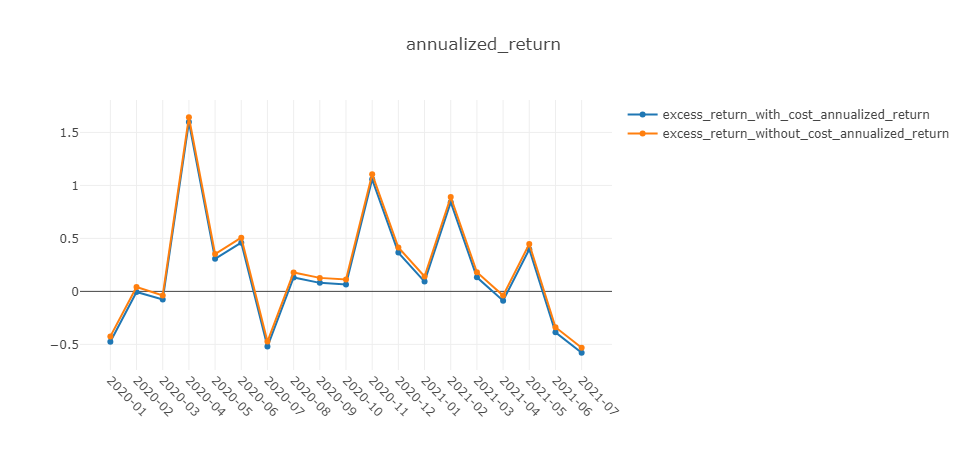
\includegraphics[width=0.4\textwidth]{annualized_return.png}
    \caption{Annualized Return (monthly)}
    \label{fig:annualized return (monthly)}
\end{figure}

As shown in Fig. \ref{fig:annualized return (monthly)}, at the most time, the strategy's monthly annualized excess return was positive, which means that the strategy outperformed the benchmark in most months.
Even though there were some months when the strategy underperformed the benchmark, the gap was not significant.

\begin{figure}[htbp]
\centering
    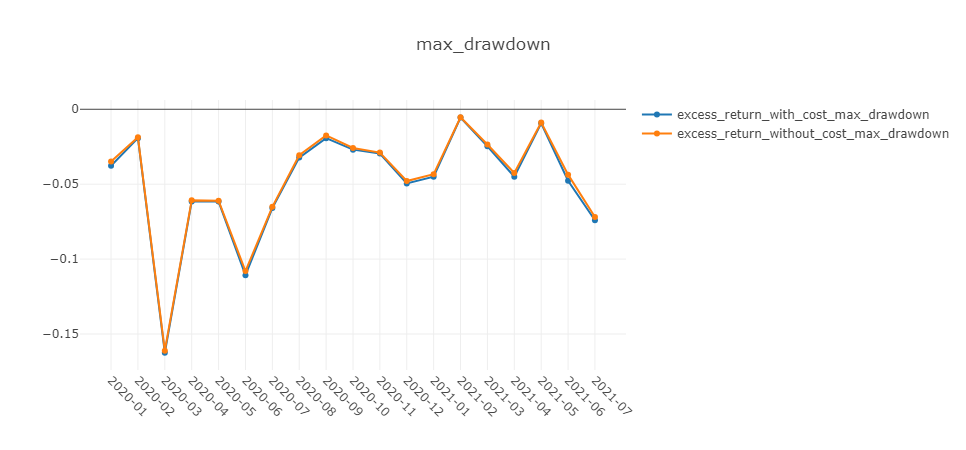
\includegraphics[width=0.4\textwidth]{max_drawdown.png}
    \caption{Maximum Drawdown (monthly)}
    \label{fig:maximum drawdown (monthly)}
\end{figure}

The excess return's maximum drawdown is shown in Fig. \ref{fig:maximum drawdown (monthly)}.
The strategy's maximum drawdown was relatively low in most months, which indicates that the strategy's risk was well controlled.
The worst month was March 2020, when the strategy's maximum drawdown reached about -0.15.

\begin{figure}[htbp]
\centering
    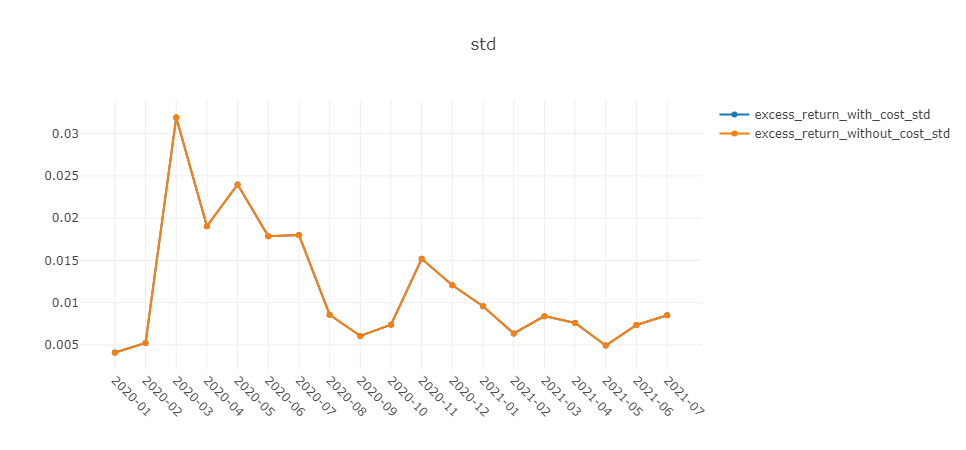
\includegraphics[width=0.4\textwidth]{std.png}
    \caption{Standard Deviation (monthly)}
    \label{fig:standard deviation (monthly)}
\end{figure}

The standard deviation of the excess return is shown in Fig. \ref{fig:standard deviation (monthly)}.
It is a measure of the strategy's risk, and relatively lower and more stable with time going on, indicating that the strategy's risk was well controlled.

\subsection{\textbf{Discussion}}

The backtesting results show that the strategy outperformed the benchmark in most months, with a positive annualized excess return and relatively low maximum drawdown, and the standard deviation of the excess return was relatively low and stable gradually.
The strategy's performance was relatively stable and well-controlled, indicating that the strategy was effective in generating excess returns while managing risk.
But sometimes the strategy underperformed the benchmark, despite the gap not being significant.

From the perspective of the market conditions, the outbreak of the COVID-19 pandemic in early 2020 caused significant market volatility, both the strategy and the benchmark experienced a significant drawdown during this period, and the strategy's excess return was negative, suggesting that the strategy may have been vunerable to the market's extreme volatility, but the risk still well controlled.
However, when the market recovered and stabilized, the strategy's performance improved significantly compared to the benchmark, suggesting that the strategy was able to generate excess returns while managing risk effectively.

Besides, the strategy's turnover rate was relatively low, indicating that the strategy was not overtrading over the backtesting period, which is a positive sign for the strategy's performance, meanwhile, cut down the transaction costs.

The backtesting results demonstrate that our comprehensive quantitative trading strategy, which integrates sentiment analysis with traditional price-volume features, can generate excess returns while managing risk effectively in the stable market conditions, even in the extreme market conditions, the risk still well controlled.
It provides a promising approach to enhancing quantitative trading strategies.

\section{\textbf{Conclusion}}

This study presents an integrated quantitative trading strategy that combines sentiment analysis with traditional price-volume features.
Using the fine-tuned Llama 3 model fine-tuned with Low-Rank Adaptation (LoRA), we efficiently processed textual data to generate sentiment factor. 
The factor, combined with traditional price-volume features, formed a comprehensive set of inputs for the LightGBM model, which was used to forecast price movements and generate trading signals to manage the portfolio.
Backtesting results showed that our strategy outperformed the benchmark (SPY) in most months, with positive annualized excess return and controlled risk. 
The strategy demonstrated resilience during the volatile period and improved performance as market conditions stabilized.

In summary, our approach effectively enhances quantitative trading strategies by integrating sentiment analysis, leading to better predictive accuracy and risk management. 
Future work could explore incorporating additional models and optimizing feature engineering processes to further improve performance.

\begin{thebibliography}{00}
    \bibitem{yang2020} X. Yang, W. Liu, D. Zhou, J. Bian, and T.-Y. Liu, “Qlib: An AI-oriented Quantitative Investment Platform.” arXiv, Sep. 22, 2020. Accessed: Jun. 21, 2024. [Online]. Available: http://arxiv.org/abs/2009.11189
    \bibitem{deng2023}X. Deng, V. Bashlovkina, F. Han, S. Baumgartner, and M. Bendersky, “What do LLMs Know about Financial Markets? A Case Study on Reddit Market Sentiment Analysis,” in Companion Proceedings of the ACM Web Conference 2023, Austin TX USA: ACM, Apr. 2023, pp. 107–110. doi: 10.1145/3543873.3587324.
    \bibitem{pavlyshenko2023} B. M. Pavlyshenko, “Financial News Analytics Using Fine-Tuned Llama 2 GPT Model.” arXiv, Sep. 11, 2023. Accessed: May 11, 2024. [Online]. Available: http://arxiv.org/abs/2308.13032
    \bibitem{hu2021} E. J. Hu et al., “LoRA: Low-Rank Adaptation of Large Language Models.” arXiv, Oct. 16, 2021. Accessed: Jun. 27, 2024. [Online]. Available: http://arxiv.org/abs/2106.09685
    \bibitem{ke2017} G. Ke et al., “LightGBM: A Highly Efficient Gradient Boosting Decision Tree”.
\end{thebibliography}

\end{document}
